\documentclass[a4paper, 11pt]{article}
\usepackage[pdftex]{graphicx}
\usepackage{fullpage}
\usepackage{mathrsfs,amsmath}


% An example of defining macros
\newcommand{\rs}[1]{\mathstrut\mbox{\scriptsize\rm #1}}
\newcommand{\rr}[1]{\mbox{\rm #1}}
% My equations
%-----------------------------------------------------------
\renewcommand{\div}{\nabla\cdot}
\newcommand{\grad}{\vec \nabla}
\newcommand{\curl}{{\vec \nabla}\times}
\renewcommand{\H}{{\vec H}}
\newcommand {\J}{{\vec J}}
\newcommand {\E}{{\vec E}}
\newcommand{\siginf}{\sigma_\infty}
\newcommand{\dsig}{\triangle\sigma}
\newcommand{\dcurl}{{\mathbf C}}
\newcommand{\dgrad}{{\mathbf G}}
\newcommand{\Acf}{{\mathbf A_c^f}}
\newcommand{\Ace}{{\mathbf A_c^e}}
\renewcommand{\S}{{\mathbf \Sigma}}
\newcommand{\St}{{\mathbf \Sigma_\tau}}
\newcommand{\T}{{\mathbf T}}
\newcommand{\Tt}{{\mathbf T_\tau}}
\newcommand{\diag}{\mathbf{diag}}
\newcommand{\M}{{\mathbf M}}
\newcommand{\MfMui}{{\M^f_{\mu^{-1}}}}
\newcommand{\MfMuoi}{{\M^f_{\mu_0^{-1}}}}
\newcommand{\dMfMuI}{{d_m (\M^f_{\mu^{-1}})^{-1}}}
\newcommand{\dMfMuoI}{{d_m (\M^f_{\mu_0^{-1}})^{-1}}}
\newcommand{\MeSig}{{\M^e_\sigma}}
\newcommand{\MeSigInf}{{\M^e_{\sigma_\infty}}}
\newcommand{\MeSigInfEtab}{{\M^e_{\sigma_\infty \bar{\eta}}}}
\newcommand{\MeSigInfEtat}{{\M^e_{\sigma_\infty \peta}}}
\newcommand{\MedSig}{{\M^e_{\triangle\sigma}}}
\newcommand{\MeSigO}{{\M^e_{\sigma_0}}}
\newcommand{\Me}{{\M^e}}
\newcommand{\Js}{\mathbf{J}^s}
\newcommand{\Mes}[1]{{\M^e_{#1}}}
\newcommand{\Mee}{{\M^e_e}}
\newcommand{\Mej}{{\M^e_j}}
\newcommand{\BigO}[1]{\mathcal{O}\bigl(#1\bigr)}
\newcommand{\bE}{\mathbf{E}}
\newcommand{\bEp}{\mathbf{E}^p}
\newcommand{\bB}{\mathbf{B}}
\newcommand{\bBp}{\mathbf{B}^p}
\newcommand{\bEs}{\mathbf{E}^s}
\newcommand{\bBs}{\mathbf{B}^s}
\newcommand{\bH}{\mathbf{H}}
\newcommand{\B}{\vec{B}}
\newcommand{\D}{\vec{D}}
\renewcommand{\H}{\vec{H}}
\newcommand{\s}{\vec{s}}
\newcommand{\bfJ}{\bf{J}}
\newcommand{\vecm}{\vec m}
\renewcommand{\Re}{\mathsf{Re}}
\renewcommand{\Im}{\mathsf{Im}}
\renewcommand {\j}  { {\vec j} }
\newcommand {\h}  { {\vec h} }
\renewcommand {\b}  { {\vec b} }
\newcommand {\e}  { {\vec e} }
\renewcommand {\d}  { {\vec d} }
\renewcommand {\u}  { {\vec u} }

\renewcommand {\dj}  { {\mathbf{j} } }
\renewcommand {\dh}  { {\mathbf{h} } }
\newcommand {\db}  { {\mathbf{b} } }
\newcommand {\de}  { {\mathbf{e} } }

\newcommand{\vol}{\mathbf{v}}
\newcommand{\I}{\vec{I}}
\newcommand{\A}{\mathbf{A}}
\newcommand{\bI}{\mathbf{I}}
\newcommand{\bus}{\mathbf{u}^s}
\newcommand{\brhss}{\mathbf{rhs}_s}
\newcommand{\bup}{\mathbf{u}^p}
\newcommand{\brhs}{\mathbf{rhs}}
%%-------------------------------
\newcommand{\bon}{b^{on}(t)}
\newcommand{\bp}{b^{p}}
\newcommand{\dbondt}{\frac{db^{on}(t)}{dt}}
\newcommand{\dfdt}{\frac{df(t)}{dt}}
\newcommand{\dbdt}{\frac{\partial \b}{\partial t}}
\newcommand{\dfdtdsiginf}{\frac{\partial\frac{df(t)}{dt}}{\partial\siginf}}
\newcommand{\dfdsiginf}{\frac{\partial f(t)}{\partial\siginf}}
\newcommand{\dbgdsiginf}{\frac{\partial b^{Impulse}(t)}{\partial\siginf}}
\newcommand{\digint}{\frac{2}{\pi}\int_0^{\infty}}
\newcommand{\Gbiot}{\mathbf{G}_{Biot}}
%%-------------------------------
\newcommand{\peta}{\tilde{\eta}}
\newcommand{\petadt}{\frac{\partial \tilde{\eta}}{\partial t}}
\newcommand{\eFmax}{\e^{F}_{max}}
\newcommand{\dip}{d^{IP}}
\newcommand{\sigpert}{\delta\sigma}


\newcommand{\SimPEG}{\textsc{SimPEG}\xspace}
\newcommand{\simpegEM}{\textsc{simpegEM}\xspace}


\begin{document}
\graphicspath{{./IPFigures/}}


\subsection{Derivation for Seigel's result}
As an intial step to get some insights of induced polarization effect, we need to start with Cole-Cole model 
\begin{equation}
\sigma(\omega)=\sigma_{\infty}(1-\eta(\frac{1}{1+(1-\eta)(\imath\omega\tau)^c})), \label{eq:2.1}
\end{equation}
\begin{align}
	\sigma_{\infty} = \frac{\sigma_0}{1-\eta}, \label{eq:2.2}\\
	\sigma_{0} = \sigma_{\infty}(1-\eta). \label{eq:2.3}
\end{align}
Constituitive relation ships in both frequency and time domain can be written as 
\begin{align}
	\J(\omega) = \sigma(\omega)\E(\omega), \label{eq:2.4}\\
	\j(t) = \sigma(t)\otimes \e(t).\label{eq:2.5}
\end{align}
Then what does the $\j(t)$ look like? Suppose $\eta=0$, then $\sigma(\omega) = \sigma_{\infty}$. Thus, 
\begin{align}
	\sigma(t) = \frac{1}{2\pi}\int_{-\infty}^{+\infty}\sigma_{\infty}e^{\imath\omega t} d\omega,\\ \nonumber
			  = \sigma_{\infty}\delta(t).\label{eq:2.6}
\end{align}
So if there is no frequency dependence $\sigma(t)$, regarded as a function, has a delta function representation. Hence, 
\begin{align}
	\j(t) = \int_{-\infty}^{+\infty}\sigma(u)e(t-u) du,\\ \nonumber
	     = \sigma_{\infty}\e(t),\label{eq:2.7}
\end{align}
that is, the current density is a scaled value of the present electric field. Now consider a chargeable body, write Cole-Cole model in frequency domain (equation~\ref{eq:2.1}), 
\begin{align}
	\sigma(\omega) = \sigma_{\infty} + \Delta \sigma(\omega),  \\ \nonumber
	\Delta \sigma(\omega) = -\sigma_{\infty}\peta^{I}(\omega),\\ \nonumber
	\peta^{I}(\omega) = \frac{\eta}{1+(1-\eta)(\imath\omega\tau)^c}. \
\end{align}
Here $\peta^{I}(\omega)$ is a small, frequency dependent quantity that comprises composite effect of $\eta$, $\tau$, and $c$. To find hows this translates to the time domain, take the inverse Fourier (or Laplace) transform. We can get an analytic expresion for $c$=1. Then 
\begin{align}
	\Delta \sigma(\omega) = -\sigma_{\infty}\frac{\eta}{1+(1-\eta)(\imath\omega\tau)^c}, \label{eq:2.9}\\
	\Delta \sigma(t) = \frac{-\eta\sigma_{\infty}}{(1-\eta)\tau}e^{\frac{-t}{(1-\eta)\tau}u(t)}, \label{eq:2.10}
\end{align}
wwhere $u(t)$ is a Heaviste step function. We presented Cole-Cole model in time domain, When $\eta=0.1$, $\tau=0.1$, $c=1$, $\sigma_0=1e-3$ $S/m$ in Figure~\ref{F:coleTD}. So the conductivity representation in the time domain is negative. The understanding is rooted in the following. The physical quantity that we are interested is current density ($\j(t)$). Suppose a constant electric field and a chargeable and non-chargeable medium. Then the conductivities in time domain can be represented as top and middle panel of Figure~\ref{F:Prej}. For non-chargeable medium, the conductivity in time domain is a delta function at $t=0$. Using equation~\ref{eq:2.5}, we can compute current density ($J$) for both cases as shown in Figure~\ref{F:Postj}. As we can expect, we may have step-off function for non-chargeable case as shown in the bottom panel of Figure~\ref{F:Postj}. However, for chargeable case, we have negative transients after $t=0$. In addait tion, negative transients before $t=0$ tells us that net current is reduced, compared to the non-chargeable case. \\
Then, what is the magnitude of the polarization current?
\begin{eqnarray}
	\j(t) = j(t=0) + \Delta \j(t) \\
	j(t=0) = j_{\sigma_{\infty}} =\sigma_{\infty}e_0 \\
	\Delta \j(t) = \Delta \sigma \otimes \e(t) = \int^{\infty}_{-\infty} \Delta \sigma(t-u) e(u) du \\
											 = \int^{0}_{-\infty} \Delta \sigma(t-u) e(u) du
\end{eqnarray}
The maximum value of $\Delta \j(t)$:
\begin{eqnarray}
	max\Delta \j = \Delta \j(t=0) = \int^{0}_{-\infty} \Delta \sigma(-u) e(u) du\\
	= \frac{-\eta\sigma_{\infty}}{(1-\eta)\tau}\int_{-\infty}^{0} e^{\frac{+u}{(1-\eta)\tau}} du\\
	Let,\ b = \frac{1}{(1-\eta)\tau}\nonumber \\ 
	\int_{-\infty}^{0} e^{bu} du = \frac{1}{b}e^{bu}|^{0}_{-\infty} = \frac{1}{b}-0 = \frac{1}{b}\nonumber \\
	So,\ max\Delta \j = - e_0\sigma_{\infty}\eta.	
\end{eqnarray}
 Thus, 
\begin{align}
	max \frac{\Delta \j}{j_{\sigma_{\infty}}} = -\eta, \\
	Let,\ max \Delta \j = \Delta \j^{pol} = -\eta j_{\sigma_{\infty}}.
\end{align}
This is Seigel's result. \\
Here we have 
\begin{align}
	j(t=0)= j_{\sigma_{\infty}}+\Delta \j(t=0) = (\sigma_{\infty}-\eta)e_0 = \sigma_0e_0,
\end{align}
where $\sigma_0$ is the conductivity at $\omega=0$.
Interestingly, for the step-on source, we have
\begin{align}
	j(t=0)= j_{\sigma_{\infty}}+\Delta \j(t=0) = \sigma_{\infty}e_0.
\end{align}
Since $\Delta \j(t=0)=0$ for the step-on case. Therefore, the initial condition for step-off source and step-on source are different. More specifically, we need to use $\sigma_0$ and $\sigma_{\infty}$ for step-off and step-on sources, respectively. We can obtain current density for step-on source by using equaton~\ref{eq:2.5}, and presented in Figure~\ref{F:Postjstepon}. We checked our derivation through initial conditions in Figures~\ref{F:Postj} and \ref{F:Postjstepon}. 

\begin{figure}[htb]
	\centering
	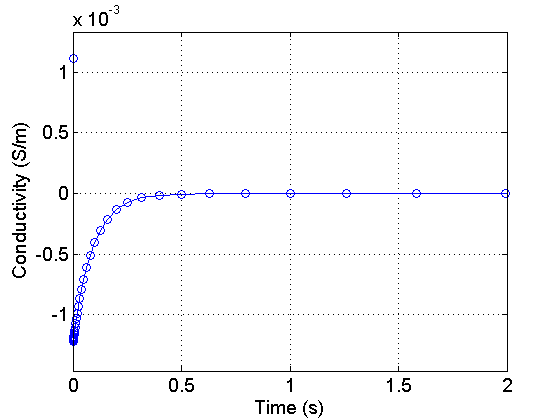
\includegraphics[width=0.6\textwidth]{coleTD.png}
	\caption{Analytic Cole-Cole model in time domain.}
	\label{F:coleTD}
\end{figure}

\begin{figure}[htb]
	\centering
	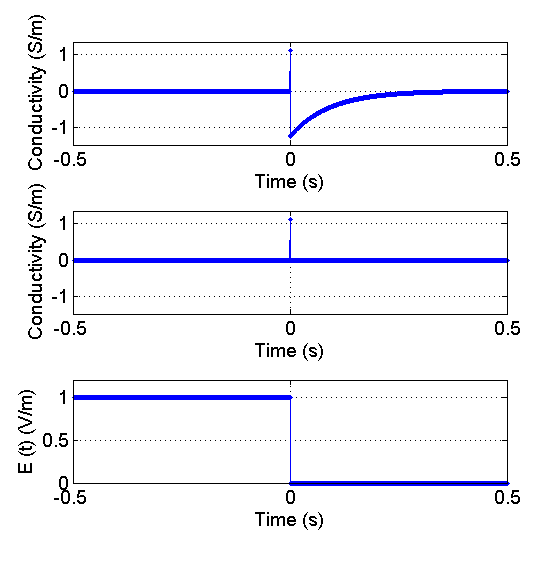
\includegraphics[width=0.6\textwidth]{PreJ.png}
	\caption{Conductivities in time domain (top panel) for chareable and non-chargeable medium (middle panel). Step-off response of electric fied (bottom panel).}
	\label{F:Prej}
\end{figure}

\begin{figure}[htb]
	\centering
	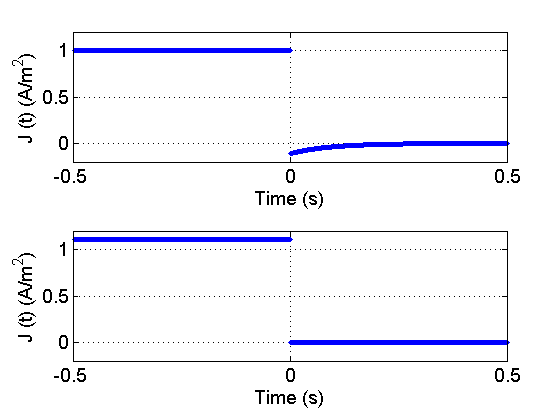
\includegraphics[width=0.6\textwidth]{PostJ.png}
	\caption{Current densities in time domain for chargeable (top panel) and non-chargeable medium (bottom panel). Here we used step-off electric field.}
	\label{F:Postj}
\end{figure}
\begin{figure}[htb]
	\centering
	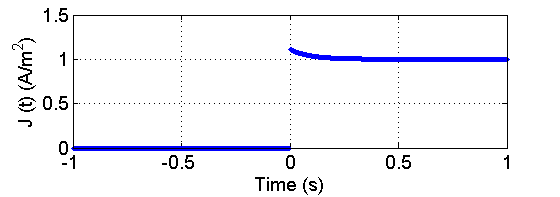
\includegraphics[width=0.6\textwidth]{PostJstepon.png}
	\caption{Current density in time domain for chargeable medium with step-on electric field.}
	\label{F:Postjstepon}
\end{figure}
\clearpage

\subsection{IP sphere problem}

\subsubsection{Electric fields}
In order to get some insights of IP responses and chage distribution, we apply complex conductivity model to the static sphere problem.
Here we can plug in complex conductivity model to $\sigma_2$. Assume that we know solutions of electric fields for a conductive sphere of radius $R$ in a uniform electrostatic case: \\
The electric field outside ($r>R$) is 
\begin{equation}
	\mathbf{E_1} = E_0\mathbf{\hat{x}}+E_0R^3\frac{\sigma_2(\omega)-\sigma_1}{\sigma_2(\omega)+2\sigma_1}\frac{(2x^2-y^2-z^2)\mathbf{\hat{x}}+(3xy)\mathbf{\hat{y}}+(3xz)\mathbf{\hat{z}}}{r^5},
\label{eq:IPspheq1}		
\end{equation}
and inside ($r<R$) is
\begin{equation}
	\mathbf{E_2} = E_0\frac{3\sigma_1}{\sigma_2(\omega)+2\sigma_1}\mathbf{\hat{x}},
\label{eq:IPspheq2}		
\end{equation}
where 
\begin{displaymath}
	\sigma_2(\omega) = \sigma_{\infty}(1-\frac{\eta}{1+(1-\eta)(\imath\omega\tau)^c}).
\end{displaymath}
To make our problem simple, we use $c=1$. Then we have
\begin{displaymath}
	\sigma_2(\omega) = \sigma_{\infty}(1-\frac{\eta}{1+(1-\eta)(\imath\omega\tau)}).
\end{displaymath}
Since we are using the time dependency, $e^{-\imath\omega t}$, we use $\sigma_2(\omega)^*$. If you think about time domain responses of equations~\ref{eq:IPspheq1} and ~\ref{eq:IPspheq2}, they are only dependent of $\sigma_2(\omega)$; thus, we substitute some related variables:
\begin{align*}
	\mathbf{E_1} = E_0\mathbf{\hat{x}}+k_1(\omega)E_0R^3\frac{(2x^2-y^2-z^2)\mathbf{\hat{x}}+(3xy)\mathbf{\hat{y}}+(3xz)\mathbf{\hat{z}}}{r^5}\\
	=E_0\mathbf{\hat{x}}+k_1(\omega)\mathbf{P} \\
	\mathbf{E_2} = E_0k_2(\omega)\mathbf{\hat{x}},\\
	k_1(\omega)=\frac{\sigma_2^*(\omega)-\sigma_1}{\sigma_2(\omega)^*+2\sigma_1},\\
	k_2(\omega)=\frac{3\sigma_1}{\sigma_2(\omega)^*+2\sigma_1}.\\
	\mathbf{P} = E_0R^3\frac{(2x^2-y^2-z^2)\mathbf{\hat{x}}+(3xy)\mathbf{\hat{y}}+(3xz)\mathbf{\hat{z}}}{r^5}
\end{align*}
We calculate step-off responses of these by using inverse Fourier transform:
\begin{align*}
	\mathbf{e}(t) = \frac{1}{2\pi}\int_{-\infty}^{\infty}\frac{\mathbf{\E(\omega)}}{\imath\omega}e^{-\imath\omega t} d\omega.
\end{align*}
The electric field out- and inside are
\begin{align*}
	\mathbf{e}_1(t) = E_0u(-t)\mathbf{\hat{x}} + k_1(t)\mathbf{P}, \\
	\mathbf{e}_2(t) = k_2(t)E_0\mathbf{\hat{x}},
\end{align*}
where
\begin{align*}
	k_1(t) = \frac{1}{2\pi}\int_{-\infty}^{\infty}\frac{k_1(\omega)}{\imath\omega}e^{-\imath\omega t} d\omega, \\
	k_2(t) = \frac{1}{2\pi}\int_{-\infty}^{\infty}\frac{k_2(\omega)}{\imath\omega}e^{-\imath\omega t} d\omega.
\end{align*}
Thus, by solving these two infinte integrals we can obtain analytic expression for IP responses for static sphere problem. 
\begin{align*}
	\frac{k_1(\omega)}{\omega}=\frac{\sigma_2^*(\omega)-\sigma_1}{\sigma_2(\omega)^*+2\sigma_1}\\
	=\frac{1}{\omega}\frac{ \sigma_{\infty}-\sigma_1-\sigma_{\infty}\frac{\eta}{1-(1-\eta)(\imath\omega\tau)} }
	                      { \sigma_{\infty}+2\sigma_1-\sigma_{\infty}\frac{\eta}{1-(1-\eta)(\imath\omega\tau)} }, \\
	=\frac{1}{\omega}\frac{ (\sigma_{\infty}-\sigma_1)1-(1-\eta)(\imath\omega\tau)-\sigma_{\infty}\eta }
	                      { (\sigma_{\infty}+2\sigma_1)1-(1-\eta)(\imath\omega\tau)-\sigma_{\infty}\eta }, \\	  
\end{align*}
Let
\begin{align*}
	a = \sigma_{\infty}-\sigma_1, \\
	b = \sigma_{\infty}+2\sigma_1, \\
	\hat{a} = \sigma_{\infty}(1-\eta)-\sigma_1, \\
	\hat{b} = \sigma_{\infty}(1-\eta)+2\sigma_1, \\
	A = (\sigma_{\infty}-\sigma_1)(1-\eta)\tau,  \\
	B = (\sigma_{\infty}+2\sigma_1)(1-\eta)\tau. 
\end{align*}
Then we have
\begin{align*}
	\frac{k_1(\omega)}{\omega}=\frac{1}{\omega}\frac{\hat{a}-A\imath\omega}{\hat{b}-B\imath\omega}
			   				  =\frac{A'}{\omega}+\frac{B'}{\omega(\hat{b}-B\imath\omega)}. \\
	A' = \frac{\hat{a}}{\hat{b}}, \\
	B' = (\frac{\hat{a}}{\hat{b}}B-A)\imath, \\
	\frac{k_1(\omega)}{\omega}=\frac{\frac{\hat{a}}{\hat{b}}}{\omega}+\frac{(\frac{\hat{a}}{\hat{b}}B-A)}{\omega(\hat{b}-B\imath\omega)}. \\
\end{align*}
Now we use Residual theorm to evaluate this complex integral. Be careful that where your singular point is located, because that gives you different contour path, which gives you different sign.
\begin{align}
	k_1(t) = u(-t)\frac{\hat{a}}{\hat{b}} + (\frac{\hat{a}}{\hat{b}}-\frac{A}{B})e^{-\frac{\hat{b}}{B}t}.
	\label{eq:IPspheq3}		
\end{align}	
Since 
\begin{align*}
	\frac{\hat{a}}{\hat{b}} = \frac{\sigma_{\infty}(1-\eta)-\sigma_1}{\sigma_{\infty}(1-\eta)+2\sigma_1}
							= \frac{\sigma_{\infty}-\sigma_1-\sigma_{\infty}\eta}{\sigma_{\infty}+2\sigma_1-\sigma_{\infty}\eta}, \\
	\frac{A}{B}	= \frac{(\sigma_{\infty}-\sigma_1)(1-\eta)\tau}{(\sigma_{\infty}+2\sigma_1)(1-\eta)\tau} 
				= \frac{(\sigma_{\infty}-\sigma_1)}{(\sigma_{\infty}+2\sigma_1)}							
\end{align*}	
Let $c=-\sigma_{\infty}\eta$,
\begin{align*}
	\frac{\hat{a}}{\hat{b}}-\frac{A}{B} = \frac{\hat{a}}{\hat{b}}-\frac{a}{b} = \frac{c(a-b)}{b(b-c)}.
\end{align*}	
Since 
\begin{align*}
	b=\sigma_{\infty}+2\sigma_1>0, \\
	c=\sigma_{\infty}\eta>0, \\
	a-b=-3\sigma_1>0, \ and \\
	b-c=\sigma_{\infty}(1-\eta)+2\sigma_1>0,
\end{align*}	
$k_1(t)$ is minus when $t>0$. Thus, 
\begin{align}
	\mathbf{e}_1(t) = (E_0\mathbf{\hat{x}}+\frac{\hat{a}}{\hat{b}}\mathbf{P})u(-t) + (\frac{\hat{a}}{\hat{b}}-\frac{A}{B})e^{-\frac{\hat{b}}{B}t}\mathbf{P} \nonumber \\
	=(E_0\mathbf{\hat{x}}+\frac{\sigma_{\infty}-\sigma_1-\sigma_{\infty}\eta}{\sigma_{\infty}+2\sigma_1-\sigma_{\infty}\eta}\mathbf{P})u(-t) + (\frac{-3\sigma_1\sigma_{\infty}\eta}{(\sigma_{\infty}+2\sigma_1)(\sigma_{\infty}(1-\eta)+2\sigma_1)})
	e^{-\frac{(\sigma_{\infty}(1-\eta)+2\sigma_1)}{(\sigma_{\infty} + 2\sigma_1)((1-\eta)\tau)}t}\mathbf{P}
	\label{eq:IPspheq4}		
\end{align}

\textbf{Things to remebmer}
\begin{enumerate}
	\item The first term in lhs of the above equation, which is defined $t<0 \ and \ t=0$, is exactly same as static case without IP. 
	\item IP response for step-off source is decaying exponentially when $c=1$.
	\item $k_1(t)$ is always minus, indepenent from in and out side of conductivity values. 
	\item Static reponses (galvanic?), which is independent from frequency, will be gone in time domain responses. 
\end{enumerate}
Similarly, we can derive time domain electric field inside of the sphere.
\begin{align*}
	\frac{1}{\omega}k_2(\omega)=\frac{1}{\omega}\frac{3\sigma_1}{\sigma_2(\omega)^*+2\sigma_1}
			   				   =\frac{3\sigma_1}{\sigma_{\infty}+2\sigma_1-\frac{\sigma_{\infty}\eta}{1-(1-\eta)\tau\imath\omega}} \\
			   				   =\frac{3\sigma_1}{\omega}\frac{1-(1-\eta)\tau\imath\omega}{(\sigma_{\infty}(1-\eta)+\sigma_2)- (\sigma_{\infty}+2\sigma_1)(1-\eta)\tau\imath\omega}.
\end{align*}
Let
\begin{align*}
	s = (1-\eta)\tau, \\
	\hat{a} = \sigma_{\infty}(1-\eta) + 2\sigma_1, \\
	\hat{b} = (\sigma_{\infty} + 2\sigma_1)s.
\end{align*}
Then we have
\begin{align*}
	\frac{1}{\omega}k_2(\omega)=\frac{3\sigma_1}{\omega}\frac{1-s\imath\omega}{\hat{a}-\hat{b}\imath\omega}
							   = 3\sigma_1(\frac{A}{\omega}+\frac{B}{\hat{a}-\hat{b}\imath\omega}), \\
	A = \frac{1}{\hat{a}}, \\
	B = \imath(\frac{\hat{b}}{\hat{b}}-s).
\end{align*}
Thus, 
\begin{align*}
	\frac{1}{\omega}k_2(\omega)= 3\sigma_1(\frac{\frac{1}{\hat{a}}}{\omega}+\frac{\imath(\frac{\hat{b}}{\hat{b}}-s)}{\hat{a}-\hat{b}\imath\omega}).
\end{align*}
Similarly, by using Residual theorem we evalute infintite integral:
\begin{align}
	k_2(t) = \frac{1}{2\pi}\int_{-\infty}^{\infty}\frac{k_2(\omega)}{\imath\omega}e^{-\imath\omega t} d\omega \nonumber\\ 
		   = u(-t)\frac{3\sigma_1}{\hat{a}}+3\sigma_1(\frac{1}{\hat{a}}-\frac{s}{\hat{b}})e^{-\frac{\hat{a}}{\hat{b}}t}
	\label{eq:IPspheq5}				   
\end{align}
Since $\hat{a},\ \hat{b},\ s>0$
\begin{align*}
	\frac{1}{\hat{a}}-\frac{s}{\hat{b}} = \frac{\hat{b}-\hat{a}s}{\hat{a}\hat{b}} 
	= \frac{(\sigma_{\infty}+2\sigma_1-\sigma_{\infty}(1-\eta)-2\sigma_1)s}{\hat{a}\hat{b}} 
	= \frac{\sigma_{\infty}\eta s}{\hat{a}\hat{b}} > 0.
\end{align*}
Thus, 
\begin{align}
	\mathbf{e}_2(t) = u(-t)E_0\frac{3\sigma_1}{\hat{a}}\mathbf{\hat{x}} 
	                + 3\sigma_1(\frac{1}{\hat{a}}-\frac{s}{\hat{b}})E_0e^{-\frac{\hat{a}}{\hat{b}}t}\mathbf{\hat{x}} \nonumber \\
	                = u(-t)E_0\frac{3\sigma_1}{\sigma_{\infty}(1-\eta) + 2\sigma_1}\mathbf{\hat{x}} 
	                + 3\sigma_1(\frac{\sigma_{\infty}\eta}{(\sigma_{\infty}+2\sigma_1)(\sigma_{\infty}(1-\eta)+2\sigma_1)})
	                  E_0e^{-\frac{(\sigma_{\infty}(1-\eta)+2\sigma_1)}{(\sigma_{\infty} + 2\sigma_1)((1-\eta)\tau)}t}\mathbf{\hat{x}}
	\label{eq:IPspheq6}		
\end{align}

\textbf{Things to remebmer}
\begin{enumerate}
	\item The first term in lhs of the above equation, which is defined $t<0 \ and \ t=0$, is exactly same as static case without IP. 
	\item Electric field induced by IP effect is always in same direction to the primary electric field. 
	\item IP response after step-off is proportional to static case (inside of sphere), factor:$\frac{\sigma_{\infty}\eta}{\sigma_{\infty}+2\sigma_1}$
\end{enumerate}

In order to verify these derivations, I compared $k_1(t)$ and $k_2(t)$ with values computed by fast Hankel transform (FHT) as shown in Figure~\ref{F:IPsphereVeri}. 
\begin{figure}[htb]
	\centering
	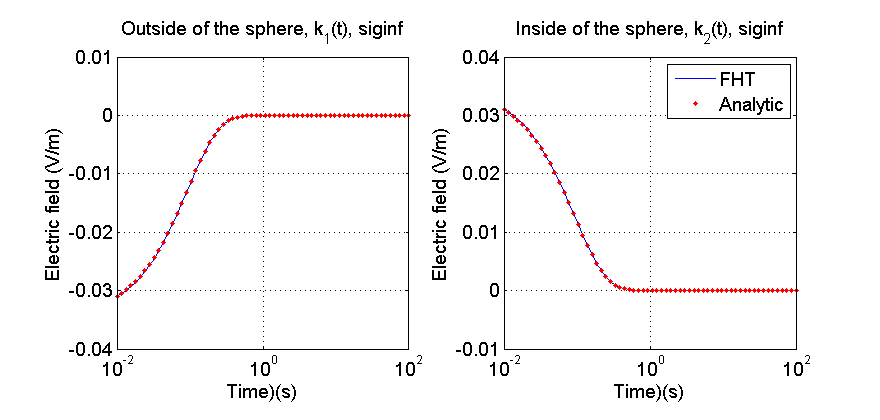
\includegraphics[width=0.8\textwidth]{IPsphereVeri.png}
	\caption{Comparison of analytic and FHT time responses for IP sphere problem.}
	\label{F:IPsphereVeri}
\end{figure}
\clearpage

\subsubsection{Charge density}

Now we can define charge distribution of the sphere as well. Consider electric field $\mathbf{e}(t>0)$, then we have
\begin{equation*}
	\nabla\cdot\epsilon\mathbf{e}(t)=\rho_v (t).
\end{equation*}
Taking volume integral for both sides and using Gauss theorem give, 
\begin{equation*}
	\int_{v}^{}	\nabla\cdot\epsilon\mathbf{e}(t) dv=	\int_{S}^{}	\rho_v(t) dv = Q(t).
\end{equation*}
Similarly, if we assume infinitesimal surface and solving the integral in above equation, we can get this relationship between two media. 
\begin{equation*}
	(\epsilon_1 e_{1}^{\perp}(t)-\epsilon_2 e_{2}^{\perp}(t)) dS = \rho_s (t) dS.
\end{equation*}
Assuming dielectric constants of two media is same gives ($\epsilon_1=\epsilon_2=\epsilon$), 
\begin{equation}
	(e_{1}^{\perp}(t)-e_{2}^{\perp}(t)) dS = \frac{\rho_s (t)}{\epsilon} dS.
\end{equation}
where $\rho_s$ is surface charge density (C/$m^2$). 
By integrating above equation on the surface of the sphere, we can calculate total charge in each hemisphere at specific time ($t>0$). Outside and inside of the normal component of electric fields at $r=R$ in spherical coordinate are given,
\begin{align*}
    e_{1}^{\perp}(t)=(\frac{-3\sigma_1\sigma_{\infty}\eta}{(\sigma_{\infty}+2\sigma_1)(\sigma_{\infty}(1-\eta)+2\sigma_1)})E_0e^{-\frac{(\sigma_{\infty}(1-\eta)+2\sigma_1)}{(\sigma_{\infty} + 2\sigma_1)((1-\eta)\tau)}t}cos\theta, \\
	e_{2}^{\perp}(t)=(\frac{3\sigma_1\sigma_{\infty}\eta}{(\sigma_{\infty}+2\sigma_1)(\sigma_{\infty}(1-\eta)+2\sigma_1)})
	                  E_0e^{-\frac{(\sigma_{\infty}(1-\eta)+2\sigma_1)}{(\sigma_{\infty} + 2\sigma_1)((1-\eta)\tau)}t}cos\theta.
\end{align*}
\begin{eqnarray*}
\epsilon\oint_{S}^{} \mathbf{e}(t)\cdot\hat{\mathbf{n}} dS=\epsilon\int_{S}^{} e_{1}^{\perp}(t)-e_{2}^{\perp}(t) dS
 =\epsilon\int_{S}^{} (e_{1}^{\perp}(t)-e_{2}^{\perp}(t)) R^2 sin\theta d\phi d\theta\\ \nonumber
 =\epsilon\int_{S}^{}  \frac{-6\sigma_1\sigma_{\infty}\eta}{(\sigma_{\infty}+2\sigma_1)(\sigma_{\infty}(1-\eta)+2\sigma_1)}
	                  E_0e^{-\frac{(\sigma_{\infty}(1-\eta)+2\sigma_1)}{(\sigma_{\infty} + 2\sigma_1)((1-\eta)\tau)}t}cos\theta R^2 sin\theta d\phi d\theta=Q(t).
\end{eqnarray*}
For the right hand side of the hemisphere, 
\begin{align*}
	2\pi\epsilon \int_{0}^{\frac{\pi}{2}} \frac{-6\sigma_1\sigma_{\infty}\eta}{(\sigma_{\infty}+2\sigma_1)(\sigma_{\infty}(1-\eta)+2\sigma_1)}E_0e^{-\frac{(\sigma_{\infty}(1-\eta)+2\sigma_1)}{(\sigma_{\infty} + 2\sigma_1)((1-\eta)\tau)}t}cos\theta R^2 sin\theta d\phi d\theta R^2 sin\theta d\theta  \\
	= \pi\epsilon\frac{-6\sigma_1\sigma_{\infty}\eta}{(\sigma_{\infty}+2\sigma_1)(\sigma_{\infty}(1-\eta)+2\sigma_1)}
	                  E_0e^{-\frac{(\sigma_{\infty}(1-\eta)+2\sigma_1)}{(\sigma_{\infty} + 2\sigma_1)((1-\eta)\tau)}t}R^2.
\end{align*}
And for the left side of the hemisphere,
\begin{align*}
	2\pi\epsilon \int_{\frac{\pi}{2}}^{\pi} \frac{-6\sigma_1\sigma_{\infty}\eta}{(\sigma_{\infty}+2\sigma_1)(\sigma_{\infty}(1-\eta)+2\sigma_1)}E_0e^{-\frac{(\sigma_{\infty}(1-\eta)+2\sigma_1)}{(\sigma_{\infty} + 2\sigma_1)((1-\eta)\tau)}t}cos\theta R^2 sin\theta d\phi d\theta R^2 sin\theta d\theta  \\
	= \pi\epsilon\frac{6\sigma_1\sigma_{\infty}\eta}{(\sigma_{\infty}+2\sigma_1)(\sigma_{\infty}(1-\eta)+2\sigma_1)}
	                  E_0e^{-\frac{(\sigma_{\infty}(1-\eta)+2\sigma_1)}{(\sigma_{\infty} + 2\sigma_1)((1-\eta)\tau)}t}R^2.
\end{align*}
Therefore, now we have conceptual model for IP-sphere case as shown in Figure~\ref{F:IPconcept}. 

\textbf{Things to remebmer}
\begin{enumerate}
	\item Charge distribution on the surface of the sphere decays in time.
	\item Polarization charge direction is independent on conductivity values of in and outside of the sphere.
\end{enumerate}
\begin{figure}[htb]
	\centering
	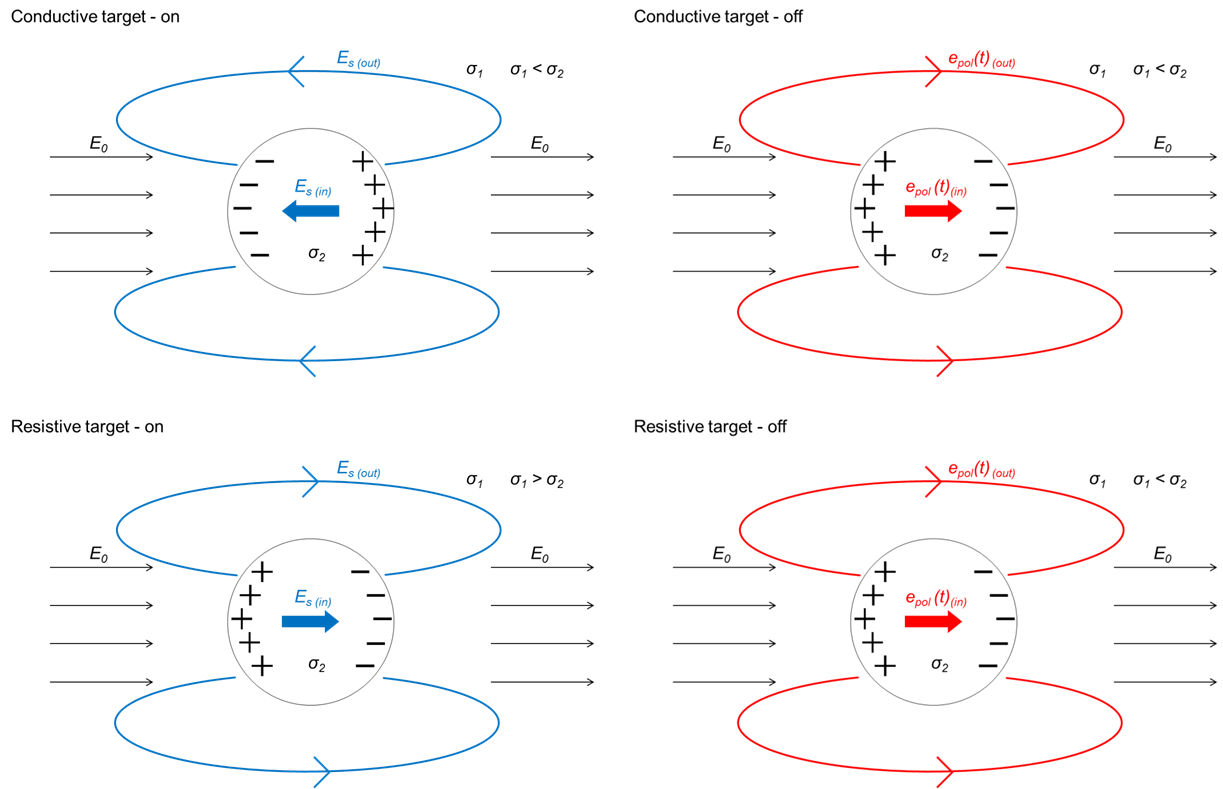
\includegraphics[width=0.9\textwidth]{ConceptModel.png}
	\caption{Conceptual model for direction of electric field and charge distribution for IP shpere problems. Here we present conductive (top panel) and resistive (bottom panel) target models.}
	\label{F:IPconcept}
\end{figure}
\clearpage
